\section{D. Irga B. Naufal Fakhri}
\subsection{Buatlah library fungsi (file terpisah/library dengan nama NPM/textunderscore bar.py) untuk plot dengan jumlah subplot adalah NPM mod 3 + 2}

Ini adalah fungsi untuk membuat plot bar sesuai dengan hasil modulus:
\lstinputlisting[firstline=8, lastline=44]{src/6/1174066/Praktek/l1174066_bar.py}

Dan ini adalah cara memanggilnya:
\lstinputlisting[firstline=7, lastline=21]{src/6/1174066/Praktek/main.py}

\subsection{Buatlah library fungsi (file terpisah/library dengan nama NPM/textunderscore scatter.py) untuk plot dengan jumlah subplot adalah NPM mod 3 + 2}

Ini adalah fungsi untuk membuat plot scatter sesuai dengan hasil modulus:
\lstinputlisting[firstline=8, lastline=44]{src/6/1174066/Praktek/l1174066_scatter.py}

Dan ini adalah cara memanggilnya:
\lstinputlisting[firstline=23, lastline=37]{src/6/1174066/Praktek/main.py}

\subsection{Buatlah library fungsi (file terpisah/library dengan nama NPM/textunderscore pie.py) untuk plot dengan jumlah subplot adalah NPM mod 3 + 2}

Ini adalah fungsi untuk membuat plot pie sesuai dengan hasil modulus:
\lstinputlisting[firstline=8, lastline=50]{src/6/1174066/Praktek/l1174066_pie.py}

Dan ini adalah cara memanggilnya:
\lstinputlisting[firstline=39, lastline=53]{src/6/1174066/Praktek/main.py}

\subsection{Buatlah library fungsi (file terpisah/library dengan nama NPM/textunderscore pie.py) untuk plot dengan jumlah subplot adalah NPM mod 3 + 2}

Ini adalah fungsi untuk membuat subplot sesuai dengan hasil modulus:
\lstinputlisting[firstline=8, lastline=44]{src/6/1174066/Praktek/l1174066_plot.py}

Dan ini adalah cara memanggilnya:
\lstinputlisting[firstline=55, lastline=69]{src/6/1174066/Praktek/main.py}


\subsection{Keterampilan Penanganan Error}
\lstinputlisting[firstline=7, lastline=19]{src/6/1174066/Praktek/1174066_error.py}
%%%%%%%%%%%%%%%%%%%%%%%%%%%%%%%%%%%%%%%%%%%%%%%%%%%%%%%%%%%%%

\section{Chandra Kirana Poetra}
\subsection{Buatlah librari fungsi (file terpisah/library dengan nama NPM bar.py) untuk plot dengan jumlah subplot adalah NPM mod 3 + 2}

\lstinputlisting[firstline=8, lastline=28]{src/6/1174079/Praktek/1174079_Bar.py}

Cara memanggilnya:
\lstinputlisting[firstline=9, lastline=17]{src/6/1174079/Praktek/main.py}

\subsection{Buatlah librari fungsi (file terpisah/library dengan nama NPM scatter.py) untuk plot dengan jumlah subplot NPM mod 3 + 2}

\lstinputlisting[firstline=8, lastline=30]{src/6/1174079/Praktek/1174079_scatter.py}

Cara memanggilnya:
\lstinputlisting[firstline=9, lastline=17]{src/6/1174079/Praktek/main.py}

\subsection{Buatlah librari fungsi (file terpisah/library dengan nama NPM pie.py) untuk plot dengan jumlah subplot NPM mod 3 + 2}

\lstinputlisting[firstline=8, lastline=29]{src/6/1174079/Praktek/1174079_pie.py}

Cara memanggilnya:
\lstinputlisting[firstline=9, lastline=17]{src/6/1174079/Praktek/main.py}

\subsection{Buatlah librari fungsi (file terpisah/library dengan nama NPM plot.py) untuk plot dengan jumlah subplot NPM mod 3 + 2}

\lstinputlisting[firstline=8, lastline=30]{src/6/1174079/Praktek/1174079_plot.py}

Cara memanggilnya:
\lstinputlisting[firstline=9, lastline=17]{src/6/1174079/Praktek/main.py}


\subsection{Keterampilan Penanganan Error}
\lstinputlisting[firstline=8, lastline=25]{src/6/1174079/Praktek/error.py}

%%%%%%%%%%%%%%%%%%%%%%%%%%%%%%%%%%%%%%%%%%%%%%%%%%%%%%%%%%%%%%%%%%%%%%%%%%%%%%%%%%%%%%%%%%%%%%%%%%%%%%%%%%%%%%%%%%%%%%%%%%

\section{Fanny Shafira Damayanti | 1174069}
\subsection{Keterampilan Pemrograman}
\begin{enumerate}
\item Jawaban NO 1
\lstinputlisting[firstline=8, lastline=30]{src/6/1174069/Praktek/1174069_bar.py}

\begin{figure}[H]
	\includegraphics[width=12cm]{figures/6/1174069/Praktek/bar.png}
	\centering
	\caption{Hasil compile membuat fungsi Bar Plot .}
\end{figure}

\item Jawaban NO 2
\lstinputlisting[firstline=8, lastline=30]{src/6/1174069/Praktek/1174069_scatter.py}

\begin{figure}[H]
	\includegraphics[width=12cm]{figures/6/1174069/Praktek/scatter.png}
	\centering
	\caption{Hasil compile membuat fungsi Scatter Plot .}
\end{figure}

\item Jawaban NO 3
\lstinputlisting[firstline=8, lastline=31]{src/6/1174069/Praktek/1174069_pie.py}

\begin{figure}[H]
	\includegraphics[width=12cm]{figures/6/1174069/Praktek/pie.png}
	\centering
	\caption{Hasil compile membuat fungsi Pie Plot .}
\end{figure}

\item Jawaban NO 4
\lstinputlisting[firstline=8, lastline=35]{src/6/1174069/Praktek/1174069_plot.py}

\begin{figure}[H]
	\includegraphics[width=12cm]{figures/6/1174069/Praktek/plot.png}
	\centering
	\caption{Hasil compile membuat fungsi Plot .}
\end{figure}

\end{enumerate}

\subsection{Penanganan Error}
Tuliskan  peringatan  error  yang  didapat  dari  mengerjakan  praktek  keenam  ini, dan  jelaskan  cara  penanganan  error  tersebut. dan  Buatlah  satu  fungsi  yang menggunakan try except untuk menanggulangi error tersebut.

\hfill \break
Peringatan error di praktek kelima ini, yaitu:
\begin{itemize}
	\item Syntax Errors
	Syntax Errors adalah suatu keadaan saat kode python mengalami kesalahan penulisan. Solusinya adalah memperbaiki penulisan kode yang salah.
	
	\item Name Error
	NameError adalah exception yang terjadi saat kode melakukan eksekusi terhadap local name atau global name yang tidak terdefinisi. Solusinya adalah memastikan variabel atau function yang dipanggil ada atau tidak salah ketik.
	
	\item Type Error
	TypeError adalah exception yang akan terjadi apabila pada saat dilakukannya eksekusi terhadap suatu operasi atau fungsi dengan type object yang tidak sesuai. Solusi dari error ini adalah mengkoversi varibelnya sesuai dengan tipe data yang akan digunakan.
\end{itemize}

\lstinputlisting[caption = Kode program membuat fungsi penanganan error., firstline=160, lastline=177]{src/6/1174069/Praktek/1174069.py}

\subsection{Screenshoot Plagiat}
\begin{figure}[H]
	\includegraphics[width=12cm]{figures/6/1174069/Praktek/plagiat.png}
	\centering
\end{figure}

%%%%%%%%%%%%%%%%%%%%%%%%%%%%%%%%%%%%%%%%%%%%%%%%%%%%%%%%%%%%%%%%%%%%%%%%%%%%%%%%%%%%%%%%%%%%%%%%%%%%%%%%%%%%%%%%%%%%

\section{Aulyardha Anindita | 1174054}
\subsection{Keterampilan Pemrograman}
\begin{enumerate}

\item Jawaban Soal No. 1
\lstinputlisting[firstline=8, lastline=29]{src/6/1174054/Praktek/1174054_bar.py}
Hasilnya adalah : 
\begin{figure}[H]
	\includegraphics[width=10cm]{figures/6/1174054/Praktek/bar.png}
	\centering
	\caption{Hasil Fungsi Bar Dita}
\end{figure}

\item Jawaban Soal No. 2
\lstinputlisting[firstline=8, lastline=30]{src/6/1174054/Praktek/1174054_scatter.py}
Hasilnya adalah : 
\begin{figure}[H]
	\includegraphics[width=10cm]{figures/6/1174054/Praktek/scatter.png}
	\centering
	\caption{Hasil Fungsi Scatter Dita}
\end{figure}

\item Jawaban Soal No. 3
\lstinputlisting[firstline=8, lastline=30]{src/6/1174054/Praktek/1174054_pie.py}
Hasilnya adalah : 
\begin{figure}[H]
	\includegraphics[width=10cm]{figures/6/1174054/Praktek/pie.png}
	\centering
	\caption{Hasil Fungsi Pie Dita}
\end{figure}

\item Jawaban Soal No. 4
\lstinputlisting[firstline=8, lastline=30]{src/6/1174054/Praktek/1174054_plot.py}

\subsection{Keterampilan Penanganan Error}

Peringatan error di praktek keenam ini, yaitu:
\begin{itemize}
\item Syntax Errors
Syntax Errors adalah keadaan dimana pada kode python mnengalami kesalahan dalam penulisan. Untuk mengatasinya yaitu dengan memperbaiki penulisan kode yang salah 

\item Name Error
NameError adalah suatu keadaan atau exception yang terjadi ketika kode melakukan eksekusi terhadap local name atau global name yang tidak terdefinisi. Untuk mengatasinya yaitu dengan memastikan variabel atau function yang dipanggil ada atau tidak salah ketik.

\item Type Error
TypeError adalah suatu keadaan atau exception yang akan terjadi apabila pada saat dilakukannya eksekusi terhadap suatu operasi atau fungsi dengan type object yang tidak sesuai. Untuk mengatasinya yaitu dengan mengkoversi varibelnya sesuai dengan tipe data yang akan digunakan.
\end{itemize}

Fungsi yang menggunakan try except
\lstinputlisting[firstline=8, lastline=25]{src/6/1174054/Praktek/error.py}
Hasilnya adalah : 
\begin{figure}[H]
	\includegraphics[width=8cm]{figures/6/1174054/Praktek/error.png}
	\centering
	\caption{Hasil Error Dita}
\end{figure}

\end{enumerate}

%%%%%%%%%%%%%%%%%%%%%%%%%%%%%%%%%%%%%%%%%%%%%%%%%%%%%%%%%%%%%%%%%%%%%%%%%%%%%%%%%%%%%%%%%%%%%%%%%%%%%%%%%%%%%%%%%%%%

\section{Nurul Izza Hamka | 1174062}
\subsection{Keterampilan Pemrograman}
\begin{enumerate}

\item Librari Fungsi Untuk NPM bar 
\lstinputlisting[firstline=10, lastline=30]{src/6/1174062/Praktek/1174062_bar.py}
Ilustrasi Gambar
	\begin{figure}[ht!]
	\includegraphics[width=10cm]{figures/6/1174062/bar.png}
	\centering
	\end{figure}

\item Librari Fungsi Untuk NPM scatter
\lstinputlisting[firstline=9, lastline=31]{src/6/1174062/Praktek/1174062_scatter.py}
Ilustrasi Gambar
	\begin{figure}[ht!]
	\includegraphics[width=10cm]{figures/6/1174062/scatter.png}
	\centering
	\end{figure}

\item Librari Fungsi Untuk NPM pie
\lstinputlisting[firstline=8, lastline=30]{src/6/1174062/Praktek/1174062_pie.py}
Ilustrasi Gambar
	\begin{figure}[ht!]
	\includegraphics[width=10cm]{figures/6/1174062/pie.png}
	\centering
	\end{figure}

\item Librari Fungsi Untuk NPM plot
\lstinputlisting[firstline=8, lastline=30]{src/6/1174062/Praktek/1174062_plot.py}
Ilustrasi Gambar
	\begin{figure}[ht!]
	\includegraphics[width=10cm]{figures/6/1174062/plot.png}
	\centering
	\end{figure}

\subsection{Penanganan Error}

\begin{itemize}

\item NameError
Error yang terjadi adalah NameError yang mana terjadi kesalahan pada saat melakukan eksekusi dan tidak dapat terdefinisi.
Penanganan yang dapat dilakukan adalah memastikan bahwa Variable dan Function yang akan kita panggil pastikan semua benar.\\

\item SyntaxError
Tipe Error ini adalah ada kesalahan pada penulisan, untuk itu pastikan penulisannya benar.\\

\item TypeError
Error ini terjadi pada saat eksekusi terhadap dan operasi dan fungsi masuk kedalam objek sedangkan typenya salah.\\

\item Menggunakan Try Except \\
\lstinputlisting[firstline=9, lastline=26]{src/6/1174062/Praktek/error.py}

\end{itemize}

\end{enumerate}

%%%%%%%%%%%%%%%%%%%%%%%%%%%%%%%%%%%%%%%%%%%%%%%%%%%%%%%%%%%%%%%%%%%%%%%%%%%%%%%%%%%%%%%%%%%%%%%%%%%%%%%%%%%%%%%%%%%%%%%%%%%%%%%%%%%
\section{Difa Al Fansha}
\subsection{Buatlah library fungsi (file terpisah/library dengan nama NPM\textunderscore bar.py|) untuk plot dengan jumlah subplot adalah NPM mod 3 + 2}
\lstinputlisting[firstline=1, lastline=71]{src/6/1174076/Praktek/1174076_bar.py}

\subsection{Buatlah library fungsi (file terpisah/library dengan nama NPM\textunderscore scatter.py) untuk plot dengan jumlah subplot adalah NPM mod 3 + 2}
\lstinputlisting[firstline=1, lastline=71]{src/6/1174076/Praktek/1174076_scatter.py}

\subsection{Buatlah library fungsi (file terpisah/library dengan nama NPM\textunderscore pie.py|) untuk plot dengan jumlah subplot adalah NPM mod 3 + 2}
\lstinputlisting[firstline=1, lastline=57]{src/6/1174076/Praktek/1174076_pie.py}

\subsection{Buatlah librari fungsi (file terpisah/library dengan nama NPM\textunderscore plot.py) untuk plot dengan jumlah subplot NPM mod 3 + 2}
\lstinputlisting[firstline=1, lastline=71]{src/6/1174076/Praktek/1174076_plot.py}

